In an actual streaming-correction run, text appears within its two-second
display deadline, then disappears for 2.176~s even though the selected
update still supports it. Certification also meets its eight-second
deadline (Figure~\ref{fig:continuity_case}(a)). Both deadline tests pass
for this interval, yet the supported result is unavailable during the
gap. Timely first delivery does not establish continued availability.

\begin{figure*}[t]
\centering
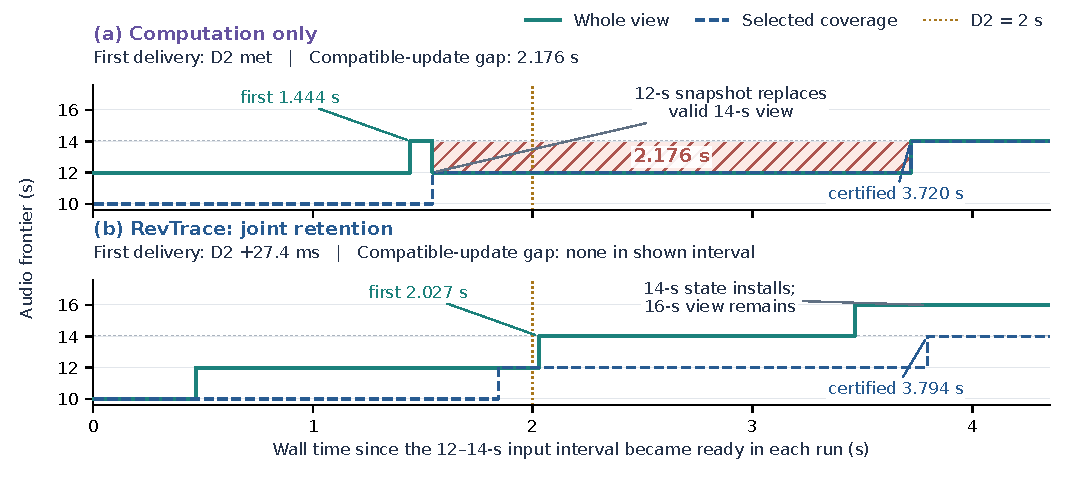
\includegraphics[width=\textwidth]{figures/timely_full_interval_case.pdf}
\caption{Timely delivery can lose supported progress. Two measured
executions of the same complete 12--14-s audio interval in a 16-session
staggered workload, each on its own service clock.
(a) Computation-only delivers 37 code points within D2, then loses the
supported view for 2.176~s before identical text returns.
(b) RevTrace delivers 27.4~ms after D2 and preserves coverage when its
14-s state installs beneath a supported 16-s view; both certified
deliveries meet C8 (8~s).}
\label{fig:continuity_case}
\end{figure*}

We study this problem in inference services whose selected outputs feed
later computation. StreamCorrect, for example, applies a learned
correction to recognition output and feeds the selected correction into
subsequent ASR~\cite{vu2026streamcorrect}. Early execution overlaps these
dependent calls, and early hypotheses can reach a consumer while
selection is still running. A selected correction must then reconcile
computation already in progress, complete results awaiting selection,
and the whole hypothesis currently being read. Preserving useful
progress requires coordinating these objects with the original feedback
program---the complete stateful call that the unmodified recognizer--corrector
pair would issue, as opposed to a stage forecast or a partial result.

The objects need different evidence. A call issued before an update can
have exactly the complete input that the update later selects, while
its own predicted successor is wrong. That call can remain useful, but
only its original correction and update may supply the selected result.
A displayed hypothesis has a separate support path: an update can
invalidate that path while a future call's input is still unresolved.
A worker executes a frozen call, an Owner serializes selected
transitions, and a Consumer maintains the current whole view.
Their decisions must preserve both valid work and the authority of the
original program.

RevTrace coordinates these decisions in one execution protocol
(Figure~\ref{fig:protocol}). It keeps unresolved full calls available
until their own inputs can be resolved, joins complete original results
to the actual selected parent, and preserves the whole visible view
when its support survives application. These are complete-call input
eligibility [EL], original selection authority [AU], and whole-view
support [SUP]. Selected facts become durable before installation; the
Consumer checks their application and reconciles its current view.
Received results remain owned independently of their producer's later
lifetime, and physical ownership is released only after terminal drain.

\begin{figure*}[t]
\centering
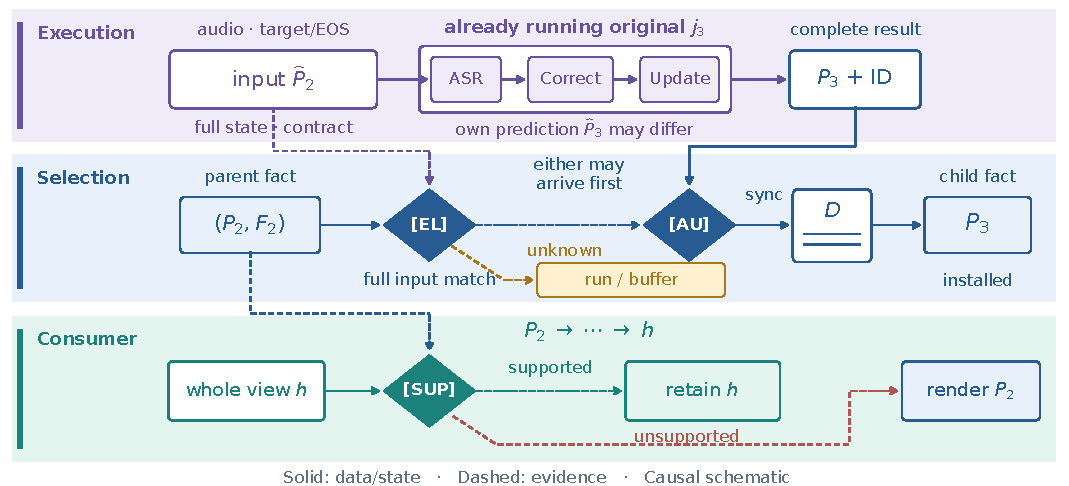
\includegraphics[width=\textwidth]{figures/coordination_protocol.pdf}
\caption{A call, its selected parent, and the Consumer's view use
evidence differently. Call $j_3$ freezes the full conditional input
before the parent's original Correct/Update selects $P_2$; a match
confirms its input while its own prediction may still differ from $P_3$.
Selection joins the complete original result with its actual parent and
owned identity, and the bound fact is synchronized before installation.
The Consumer independently checks the whole view when each fact is
applied. Pending calls may run or buffer without selection. Protocol
schematic, not a measured timing trace.}
\label{fig:protocol}
\end{figure*}

The design builds on dependency tracking, input-bound versions, and
validation before use~\cite{schlangen2011incremental,hammer2014adapton,hammer2015names}.
RevTrace combines them with original neural selection and whole-view
reconciliation so that retained computation becomes supported service.
A version bound to the complete call input supplies the same eligibility
witness: our version-DAG control shares the core input, retention,
selection, and support conditions, and its matching native handovers
show that the coordination admits multiple implementations.

The joint objective has a measurable consequence. In the prespecified
24-speaker Qwen setting with 2-s feedback and staggered arrivals,
computation retention raises total withdrawals from 12 to 17, including
avoidable withdrawals from 6 to 17, while ending the withdrawals that
later feedback itself forces. Retaining valid computation alone
nearly triples avoidable withdrawals for a simple reason: without
retention a speculative branch advances at most one step past the
certified frontier, whereas with it the branch runs several windows
ahead, so installing a compatible 12-s snapshot beneath a displayed
14-s view erases supported text unless the Consumer reconciles that
view (Figure~\ref{fig:continuity_case}(a)). View retention alone
eliminates avoidable withdrawals but delivers 628.435~s of
audio within both deadlines; joint retention delivers 680.760~s with
zero withdrawals. Preserving computation does not by itself preserve
the compatible view, and preserving the view does not recover discarded
computation.

A separate native comparison repeats both switches under the original
recognizer--corrector task, with a policy that issues nothing before
confirmation. All policies use the same two complete FP32 workers,
selection and view-support checks, and dispatcher. Across eight speakers,
in-flight retention delivers \NativeFullCreditPct\% dual-deadline
coverage against \NativeReadyCreditPct\% for completed-result reuse and
\NativeConsCreditPct\% for serial execution. Replacing the view instead
of keeping it clears all ten supported views that retained calls meet,
and buys 1.000~audio-s; keeping it erases none. Retention reduces
worker occupation by 31.8\% and two-board energy by 23.7\% against reuse;
against serial execution it spends 12.6\% more worker time for 7.4\%
less energy, serving the stream earlier rather than doing less work.

We make three contributions:
\begin{itemize}
\item \textbf{A dependability problem and service contract.} We identify
  avoidable withdrawal of supported progress after timely first
  delivery, and define the call, selected-result, and whole-view
  objects needed to distinguish continued availability from first
  arrival (Sections~\ref{sec:contract}--\ref{sec:continuation}).
\item \textbf{An executable joint protocol.} Complete-input witnesses,
  durable original selection, independent Consumer reconciliation,
  and physical ownership rules coordinate retention. Each session's
  selected facts form an execution allowed by the original program;
  replay adds no original transition. A selected-trace argument and
  executable checks establish these properties
  (Sections~\ref{sec:continuation}--\ref{sec:protocol}).
\item \textbf{Mechanism and end-to-end evidence.} Factorial controls
  expose the interaction between work retention and visible
  continuity. Native full-program comparisons measure the
  recomputation avoided by in-flight retention, with complete resource
  accounting, process-failure checks, and same-resource multi-session
  controls (Section~\ref{sec:eval}).
\end{itemize}
